\section{Use-Case}
\label{sect:useCase}

To demonstrate the cit-storm framework, a twitter stream is analyzed. This section gives a details description about all operatos used and how they are sticked together. Each operator describe above are provide by the cit-storm framework and can be combined with each other to form a meaningfull topology. In this work we analyze the twitter stream in a real-time fashion to find significant users and if once detected all following tweets are stored in a cassandra database. Tweets are split up into single words and only words from an internal badwords-table filtered to computate a user-tweet significance and finally added to a total user-significance. \newline

Figure 1 shows the final topology which uses the most of all operators. The Topology consists of two different data streams originatd at the twitter streaming source. The upper stream is responsible to keep a tweet inside the network as long as the tweet is analyzed, what is realized by an delayed-operator. The stream on the bottom analyze the tweets by linking different operators to each other. The first flatmap operator splits each tweet into single words and join these with an internal hashmap to filter only words which belongs to a word-list of interest.

\begin{figure}[h]
  \centering
  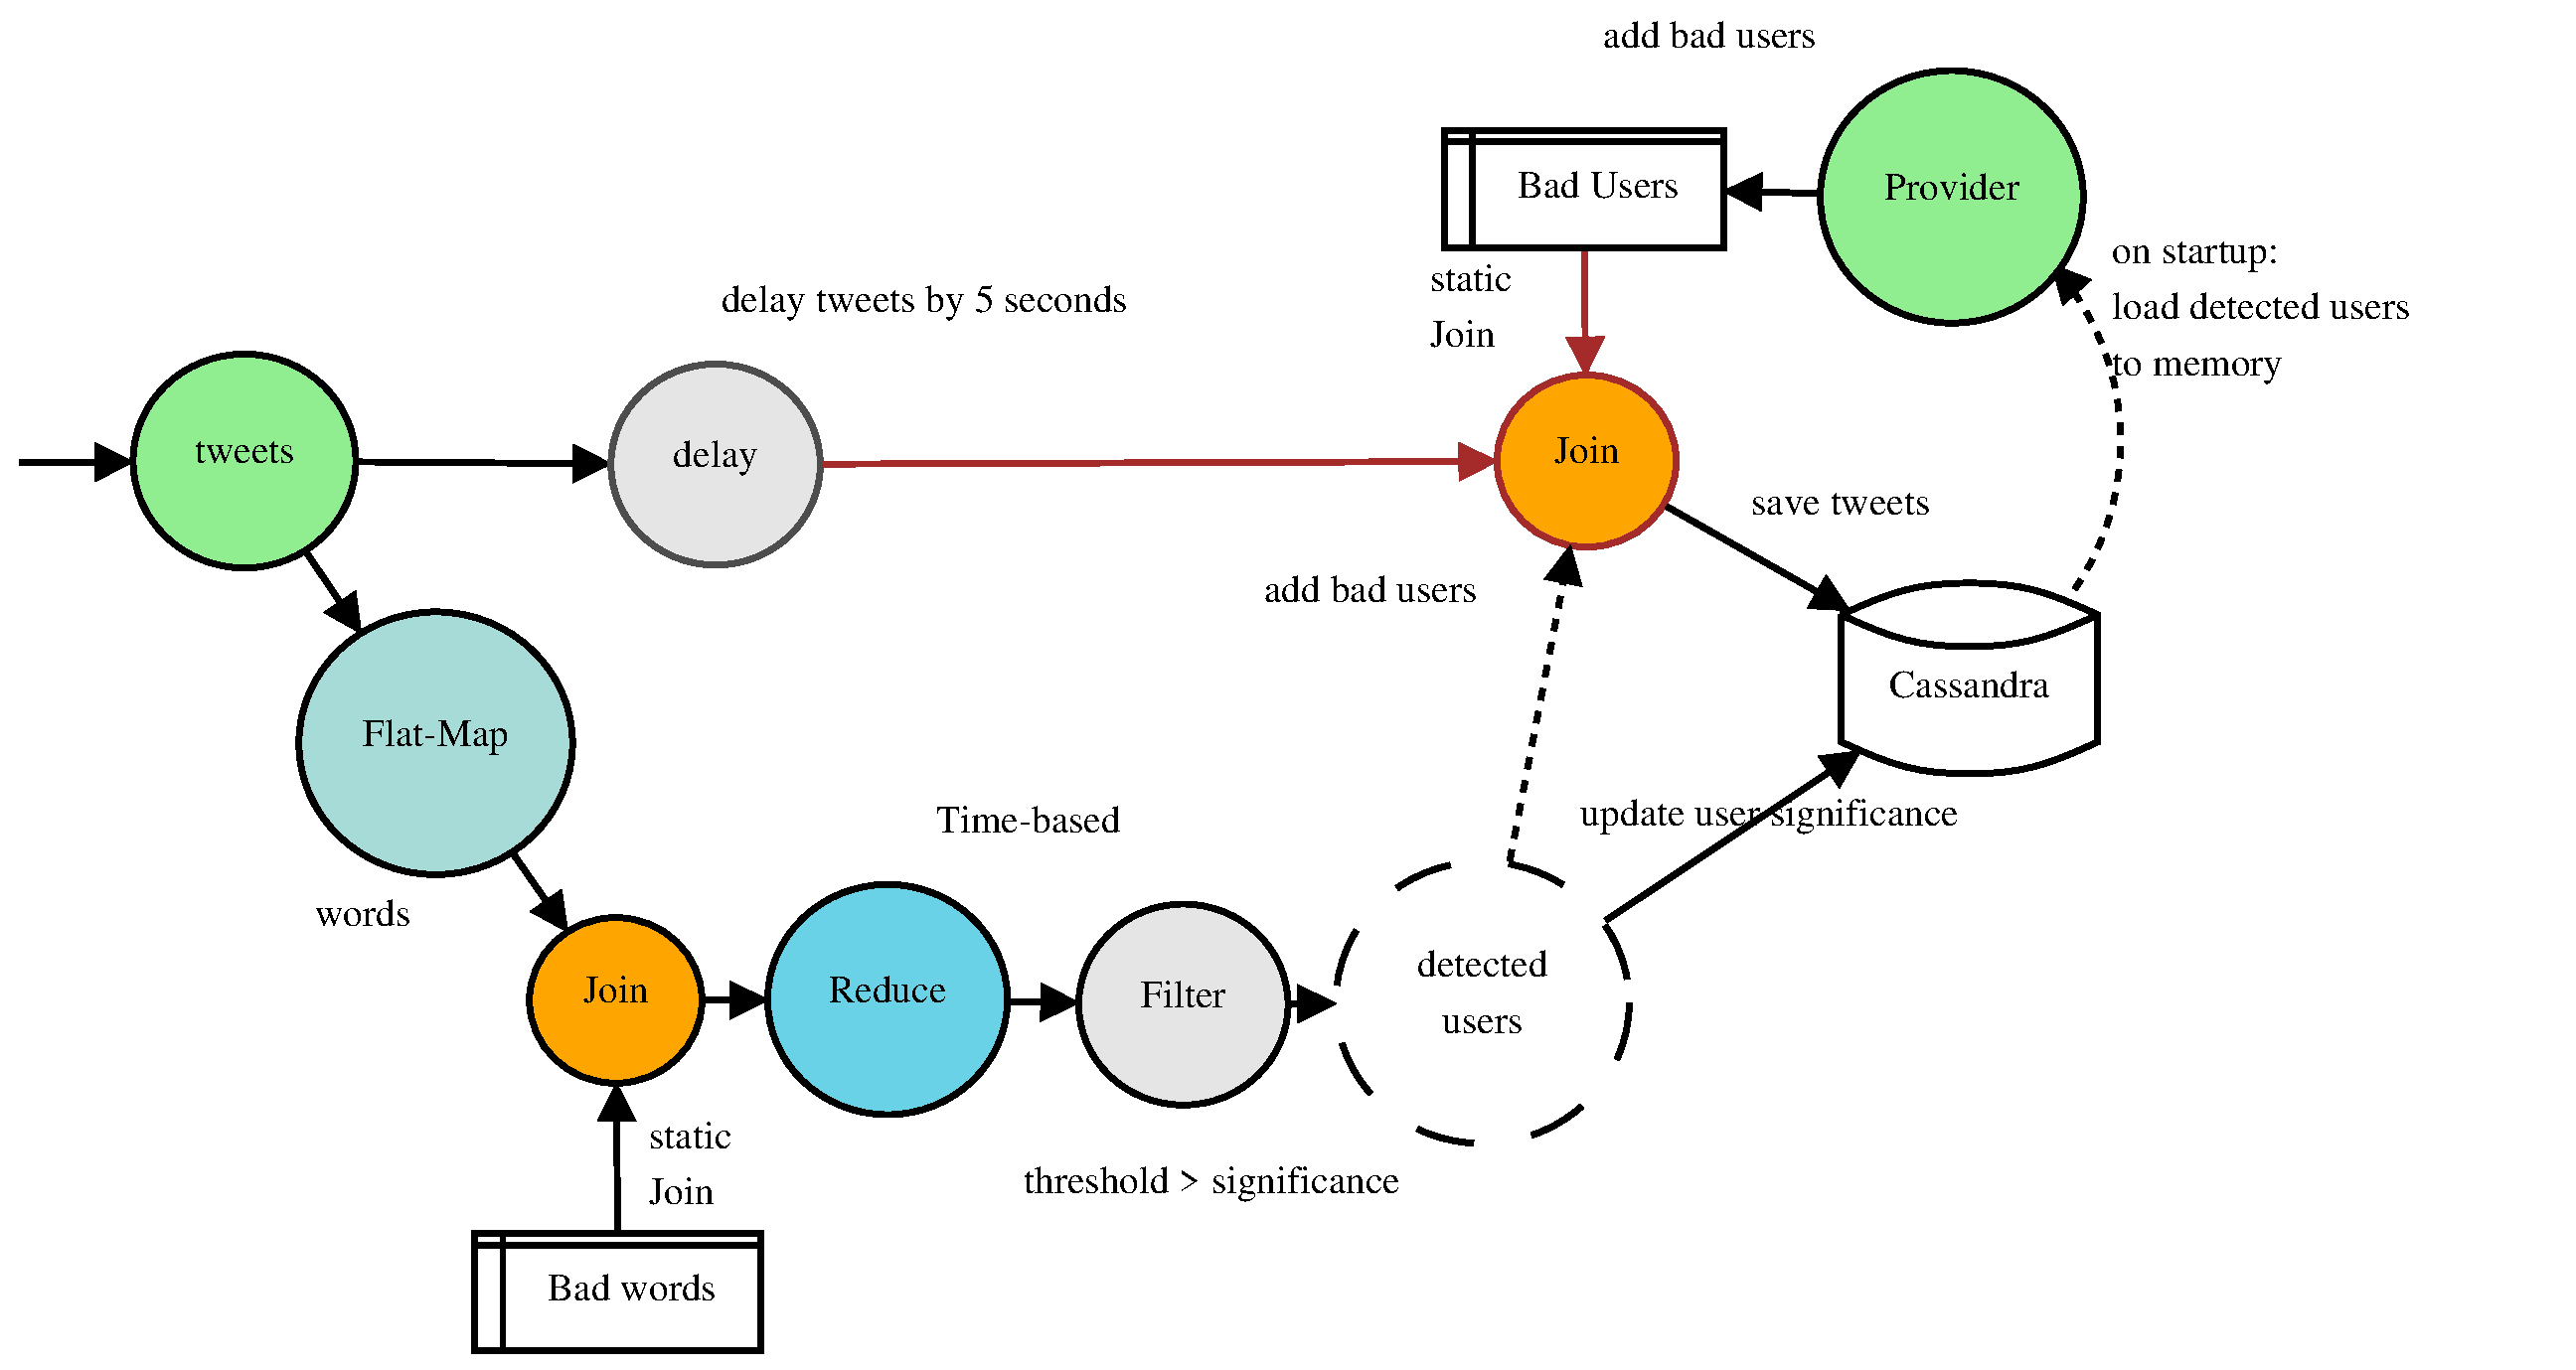
\includegraphics[width=0.6\textwidth]{images/AnalyzeTweetsTopology}
  \caption{This figure shows operators used in the topology and how they are related to each other. Operators are depicted as filled circles, in-memory storage is depicted as rectangles and dotted circles describe outputs within an operator for clarification.}
\end{figure}

\subsection{Stream semantics}

\subsubsection{Path 1: Hold tweets}


\subsubsection{Path 2: Analyze Tweets}

\subsubsection{Join}


\subsection{Cassandra Schema}
As an persistent storage cassandra is used to store detected users with its significance and their tweets. The cassandra-operator supports two different modes how to store data into the database. The \keyword{no-counter} mode assigns a specific primary-key to the incoming tuples an puts into a table. The \keyword{counter} mode only allows the increment a specific coulmn field determined by a primary-key.  

\begin{description}
  \item[user\_significance] \textit{counter} \hfill \\
  This tables stores for each user its significance-level which is increased over time. This table contains two columns, the twitter \keyword{user} and its \keyword{significance}. This table is loaded into the topology after an crash or an cluster-restart happened.
  
  \item[user\_tweets] \textit{counter}  \hfill \\
  This table stores the tweets for each user. The primary-key is \keyword{user} and \keyword{tweet\_id} with fields \keyword{tweet}.
  
  \item[word\_count]  \textit{non-counter} \hfill \\
  This table counts word occurences of bad words resulting in an user-update. The table provide some overall statistics.
  
\end{description}
    